% Template for a Computer Science Tripos Part II project dissertation
\documentclass[12pt,a4paper,twoside,openright]{report}
\usepackage[pdfborder={0 0 0}]{hyperref}    % turns references into hyperlinks
\usepackage[margin=25mm]{geometry}  % adjusts page layout
\usepackage[export]{adjustbox}
\usepackage{graphicx}  % allows inclusion of PDF, PNG and JPG images
\usepackage{verbatim}
\usepackage{docmute}   % only needed to allow inclusion of proposal.tex
\usepackage{array}     % for tables
\usepackage{nameref}
\usepackage{csquotes}

\graphicspath{ {Images/} }
\raggedbottom                           % try to avoid widows and orphans
\sloppy
\clubpenalty1000%
\widowpenalty1000%

\renewcommand{\baselinestretch}{1.1}    % adjust line spacing to make
                                        % more readable

\begin{document}

%%%%%%%%%%%%%%%%%%%%%%%%%%%%%%%%%%%%%%%%%%%%%%%%%%%%%%%%%%%%%%%%%%%%%%%%
% Title


\pagestyle{empty}

\rightline{\LARGE \textbf{George Andersen}}

\vspace*{60mm}
\begin{center}
\Huge
\textbf{QWOP in JavaScript} \\[5mm]
Computer Science Tripos -- Part II \\[5mm]
Robinson College \\[5mm]
\today  % today's date
\end{center}

% \vspace{5mm}

% \newpage
% \section*{Declaration}

% I, George Andersen of Robinson college being a candidate for Part II of the Computer Science Tripos, hereby declare that this dissertation and the work described in it are my own work, unaided except as may be specified below, and that the dissertation does not contain material that has already been used to any substantial extent for a comparable purpose.

% \bigskip
% \leftline{Signed George Andersen}

% \medskip
% \leftline{Date \today}

% %%%%%%%%%%%%%%%%%%%%%%%%%%%%%%%%%%%%%%%%%%%%%%%%%%%%%%%%%%%%%%%%%%%%
% Introduction (intro+prep ~3000)
\chapter{Introduction}
\section{What is QWOP?}
As described in the project proposal, my project is to recreate QWOP using JavaScript.
QWOP is a browser video game created by Bennett Foddy. The goal of the player is to complete a 100m race without falling over.
Figure \ref{startScreen} shows the screen on game start.
% fig of starting screen
\begin{figure}[htbp]
	\centering
	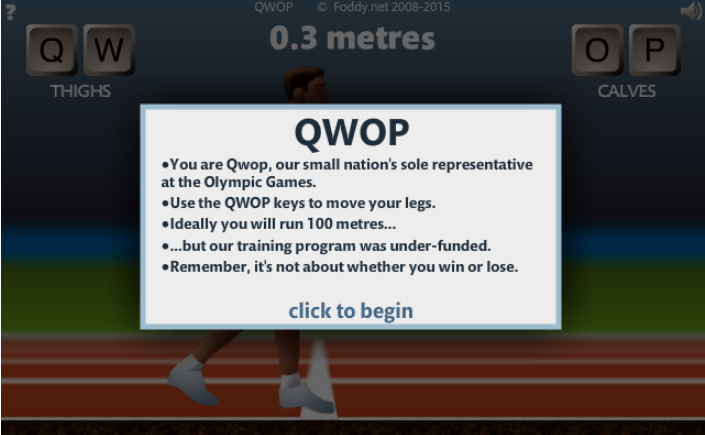
\includegraphics[width=0.7\textwidth]{startScreen.PNG}
	\caption{Starting screen of QWOP}
	\label{startScreen}
\end{figure}
Players control the athlete using only the Q, W, O, and P keys. 
Whilst the Q key is held down, the runner's right thigh is driven forward and his left thigh is driven backward. This moves the legs apart at the bottom of the torso in a scissor-like motion. 
The W key does the opposite of this, and holding it down will put the athlete in a similar stance but with his outstretched legs reversed.
The O and P keys have a similar effect but instead power the movement of the calves. The O key applies a force that moves the left calf towards the back, and the right calf forwards until it is in line with the thigh. Again the P key is the reverse of this.

Once the player clicks on the screen they are free to press the keys to attempt to move forwards. This invariably leads to Figure \ref{fallen} which shows the athlete fallen over. 
\begin{figure}[htbp]
	\centering
	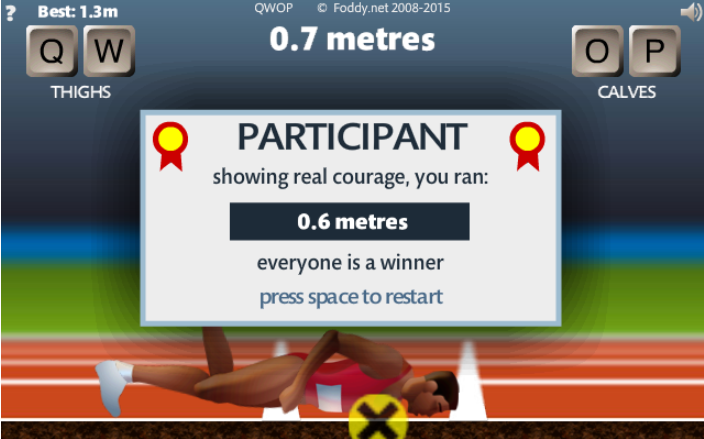
\includegraphics[width=0.7\textwidth]{qwopFallen.PNG}
	\caption{The athlete has fallen over so the player must restart.}
	\label{fallen}
\end{figure}
Below the athlete there is an X symbol. This shows where the athlete first touched the floor with his arms or head. These section of his body are not allowed to touch the floor as doing so counts as falling over. After this the player can press space and start again.
Most players attempt to keep the athlete upright and work out a key combination that will move the athlete in a motion as close to a normal gait as possible.
Others however manoeuvre the runner into a stable position on the floor, and then press lots of keys in the hope that there is a net movement forward.
Both these methods are entertaining and give some success.
Though the objective of QWOP is simple, it has been notorious for being difficult to master ever since it went viral in 2010.




% %%%%%%%%%%%%%%%%%%%%%%%%%%%%%%%%%%%%%%%%%%%%%%%%%%%%%%%%%%%%%%%%%%%%
% Preparation (intro+prep ~3000)
\chapter{Preparation}
\section{section 1}

In this chapter I will discuss the preparation that happened before the implementation of the project began.


\section{Mathematical model of the QWOP world}
\label{mathModel}
% Model needed explanation
To create QWOP in a physics simulation it first helps to know how it is going to be modelled. So when preparing it was important to first design a mathematical model of the QWOP world that could later be implemented in a physics simulation.

\subsection{Planar rigid body mechanics}
\label{prbm}

The basis of this model is planar rigid body dynamics.
% https://en.wikipedia.org/wiki/Rigid_body_dynamics
As the floor that the athlete is standing on and the limbs of the athlete do not change size and do not need to deform, they can be modelled as rigid bodies.
Save the floor, each of these rigid bodies represent one section of the athlete that has it's own position and rotation. For example the foot, upper leg and lower leg.
%should insert some rbd formulas somewhere here?
Planar rigid body mechanics uses kinematics, and solves the equations of motion described by Newton's second law to determine the motion of the bodies in the system.
%The acceleration, velocity and position of the rigid bodies can be determined using kinematics, and by solving the equations of motion described by Newton's second law.
Since this model can describe the acceleration, velocity and position of the individual rigid bodies over time, the development of the system as a whole under gravity can be simulated.
% Finish this next
With only basic planar rigid body dynamics, the limbs will just fall to the floor. So next I will describe some extensions to this model that will be made to emulate the behaviour of QWOP.

\subsection{Joints}
\label{sub:joints}

% Joints explanation
Adjacent sections are connected by joints. For example the foot and lower leg are connected at the heel, and the lower leg and upper leg are connected at the knee.
This is a constraint that the joints force the members to follow. For each joint-body connection, the joint stays in the same position relative to the frame of reference of the body - joints keep a consistent offset from each connected member. For example, the heel is always at the back of the foot, and the heel is always at the bottom of the lower leg. These two constraints work together in each joint to connect two limbs.

% Angle limiting explanation
Another constraint the joints keep is that the angle the joints rotate to is limited. For example the knee allows the lower leg to rotate up until the point where the knee is locked out. In the same way the joints in the model limit the angle they can rotate to.

\subsection{Collisions}
\label{sub:collisions}
% Collision boxes
A final constraint the limbs follow is that they collide with the floor.
Each rigid body has an area, and the areas of the limbs and the area of the floor cannot overlap, otherwise the athlete would fall through the floor.
For this reason the model needs to take collisions between the limbs and floor into account. The collisions between the limbs do not however need to be taken into account, as one limb can go behind another in the 2D view the user can see.
To model this each rigid body can have a rectangular collision box, specified by a width and height. The boxes for the limbs can then be stopped from entering the box for the floor.

% So far rigid bodies and joints
The QWOP world so far amounts to a set of rigid bodies and a set of joints on which the physics rules of planar rigid body dynamics can be applied.
The set of rigid bodies will contain 13 in total; firstly a foot, lower leg, upper leg, lower arm and upper arm for each side of the body, and also a torso, head and finally the floor. Each of these have a width and height that define their collision box, a starting position, and a mass.
The values of these variables are such that the floor is immoveable and spans the bottom of the world, and the attributes of the rigid bodies match the attributes of the limbs of the QWOP athlete.
The set of joints contains 11 in total; a left and right heel, knee, hip, shoulder, elbow, and a neck. Each of these specify which two rigid bodies they join together, the offset from each of those bodies that the joint must stay, and the maximum and minimum angles between which the joints can rotate. These connect the limbs together in the right order and keep them together with the physical properties of an athlete.


This model so far delivers an athlete with limbs that can rotate freely, move in Cartesian space and has correct joint constraints and collision checking. The last thing to add is the 

forces
rubber?

\section{Understanding Phaser}
\label{phaser}

As decided in the Project Proposal, I used Phaser to create my JavaScript version of QWOP.
One of the first things that I did to prepare was to start learning how Phaser works.
Here I shall give a brief description of what Phaser is and how it works.

Phaser is a Desktop and mobile HTML5 game framework that is designed to take care of the mundane tasks involved with developing a game so that development can be sped up. It helps keep focus on the creative aspect of game design as time is not wasted on reinventing the wheel.

Phaser handles jobs such as creating the canvas the game will be drawn to, and provides frameworks that handle compatibility issues. For example it provides access to simple methods for drawing graphics onto the canvas, and responding to user input, whether on a mobile device with a touch screen, or on a desktop with a keyboard and mouse.
%It also organises execution flow around the program and 

To take advantage of these features, a developer first imports the Phaser library by adding the minified script to their web page. %using this html code:


\begin{displayquote}
	\texttt{<script type="text/javascript" src="js/phaser.min.js"></script>}
\end{displayquote}

It is then possible to start off ones JavaScript code with a line similar to this:

\begin{displayquote}
	\texttt{var game = new Phaser.Game(gameWidth, gameHeight, Phaser.CANVAS, 'game-name', { preload: preloadFunction, create: createFunction, update: updateFunction, render: renderFunction});}
\end{displayquote}

This code shows how the Game object is created.
% I shall explain this code as it explains Phaser.
The Game object is the main controller for the entire Phaser game. 
First of all it handles the boot process. The boot process creates the canvas dimensioned to the width and height parameters provided and initialises Objects and data structures that will be used later.
After it has initialised the game, control flow is passed to code the developer has written. 
Phaser simplifies controlling the execution flow over the lifetime of the game.
It does this by giving the developer access to execute code at key moments in execution, so that the user doesn't have to write a lot of boilerplate code to organise this themselves.

The user specifies which code should be executed where using the JavaScript object passes as argument 4.
One of its key-value pairs is \texttt{update:updateFunction} so the identifier \texttt{updateFunction} is given to be used for Phaser's \texttt{update} operation. This means that the contents of updateFunction will be run once every frame.
In a similar way the developer can write a \texttt{preload} function that loads assets before the game starts that will be run at the beginning of the game.

\subsection{Sprites}

Another feature of Phaser is its use of sprites.
In the Phaser documentation \footnote{definition from https://photonstorm.github.io/phaser-ce/Phaser.Sprite.html}
sprites are described like so:

\begin{displayquote}
`At its most basic a Sprite consists of a set of coordinates and a texture that is rendered to the canvas. They also contain additional properties allowing for physics motion (via Sprite.body), input handling (via Sprite.input), events (via Sprite.events), animation (via Sprite.animations), camera culling and more.'
\end{displayquote}

\subsection{Statistical tests}

% https://www.graphpad.com/support/faqid/1790/
To prepare for the evaluation I investigated some statistical tests. 
Since lots of data is going to be collected in the evaluation, 
statistical tests needed to be compared to find appropriate ways of comparing this data.

For example to compare the distance reached for the two games, a t-test would be inappropriate 
as the participants are trying to go forwards and so the distances reached will likely not be from a Gaussian.
since data will likely not be paired,

todo: keep writing this - add other ideas used in eval and how prepped

todo: make more graphs with the orderings, work out the t test and write that up in the prep.


Next I learnt how to do these thingys
stuff in course
	stats test
	open coding?

In this chapter, I have discussed the theory that had to be understood, and work that
had to be done, before implementation could begin




%%%%%%%%%%%%%%%%%%%%%%%%%%%%%%%%%%%%%%%%%%%%%%%%%%%%%%%%%%%%%%%%%%%%
% Implementation ~4500
\chapter{Implementation}
This section details the implementation of the mathematical model of QWOP 
designed in Section \ref{mathModel}, and the implementation of the evaluation scaffolding used during the user study.
Section \ref{sec:qwopImp} focuses on the implementation of QWOP
(need to add what other subsections do).
Section \ref{studyimpl} explains the code written to produce and analyse the results of the user study.
(again add subsections of this once done) 

todo: rewrite chapter, fit with prep

% This chapter describes the implementation of the project, moving on from preparation in previous chapters. The main implementation tasks in the project were writing my version of QWOP, and writing the set of software used to perform the user study and evaluate the project. These can be divided as follows:

% \begin{itemize}
%   \item Section \ref{sec:qwopImp} \nameref{sec:qwopImp}
% 	\begin{itemize}
%       \item Section \ref{sec:jointsInPhysics} \nameref{sec:jointsInPhysics}
%   	  \item Section \ref{sec:athleteModel} \nameref{sec:athleteModel}
%   	  \item Section \ref{sec:graphics} \nameref{sec:graphics}
%   	  \item Section \ref{sec:gameFlow} \nameref{sec:gameFlow}
% 	\end{itemize}
%   \item Section \ref{studyimpl} \nameref{studyimpl}
%    \begin{itemize}
%       \item Section \ref{sec:webPage} \nameref{sec:webPage}
%       \item Section \ref{sec:serverSoftware} \nameref{sec:serverSoftware}
%       \item Section \ref{sec:chromeExtension} \nameref{sec:chromeExtension}
%     \end{itemize}
% \end{itemize}

\section{Phaser Implementation of QWOP}
\label{sec:qwopImp}
Phaser is a JavaScript framework designed for making games. I have described how it works in the preparation section, and will now break down how it was used to make the different sections of the game.


\subsection{Modelling joints in physics}
\label{sec:jointsInPhysics}
The first hurdle was to work out how to create a body in Phaser's physics engine.   
\ref{swingingRods} shows my first prototype for modelling joints and limbs, each rod is a sprite, and the joints between them are fixed together by Phaser's 'revoluteContraint's. This allows them to swing freely.

\begin{figure}[tbh]
\centerline{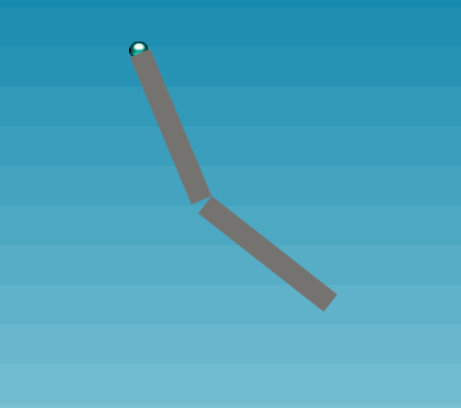
\includegraphics[scale=0.5]{swingingRods.PNG}}
\caption{Swinging rods initial model of limbs}
\label{swingingRods}
\end{figure}

The next step was make the joints apply forces to each other. This would be used to not only move the limbs when the user presses the keys, but also provide forces so that the body would stay in a similar position when keys are not pressed.

The way I did this was to use Phaser's motors on the joints. These work by applying the force needed to move the joint at the specified speed, capped off at a max value. This way of powering joints could also be used easily to apply the static forces by setting the speed to 0.

%%%%%%%%%%%%%%%%%%%%%%%%%%%%%%%%%%%%%%%%%%%%%%%%%%%%%%%%%%%%%%%%%%%
% Older versions

% https://cdn.rawgit.com/gla23/Part2Project/b43f453d1597b3f8080149ee5ca01760d64828dc/QWOPjs.html
% swinging rods

% https://cdn.rawgit.com/gla23/Part2Project/2b6292ed7cc0cb4994fea7af4697a1c1091b484d/QWOPjs.html
% 1 leg 

% https://cdn.rawgit.com/gla23/Part2Project/90935e3f9d1c2ff3d96cb271449743c98e651588/QWOPjs.html
% body without graphics

%https://cdn.rawgit.com/gla23/Part2Project/a76f298dcf66717188357c85e1b0b7667cea8e46/myQWOPjs.html
% with graphics

\subsection{Modelling the athlete}
\label{sec:athleteModel}
To model the athlete from these sprite joints, I specified the dimensions, mass, offset and starting rotation of each limb. Then forward kinematics is used on this data to get the starting points of the limbs. The limbs are then instantiated in these starting positions with the correct mass, dimensions and 'revoluteConstraint' joints. 
These joints are given joint limits so that each limb has a realistic range of motion, for example the knee joint doesn't let your lower leg rotate all the way round.
The motors for these joints are then attached to the user input according to the control scheme. If a key is pressed that powers the limb, the motor is set to the limb power, otherwise it is set to 0 so that the static forces apply.

Each limb is given a group so that materials 
either part of the  or  group, that 

\begin{figure}[tbh]
\centerline{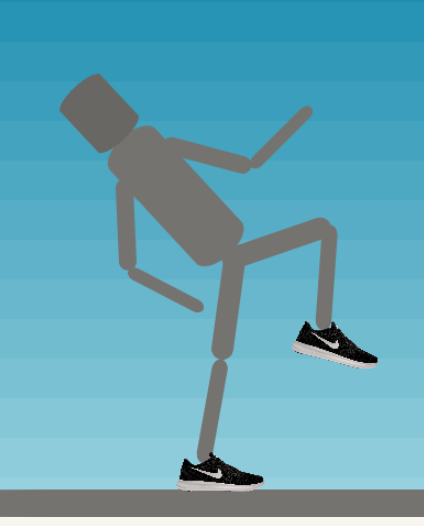
\includegraphics[scale=0.5]{athleteModel.PNG}}
\caption{Model of athlete}
\label{athleteModel}
\end{figure}

\subsection{Graphics}
\label{sec:graphics}
Next the graphics were added to the model so that it looked similar to the original QWOP.
Each sprite was given an image taken from the original.

\begin{figure}[tbh]
\centerline{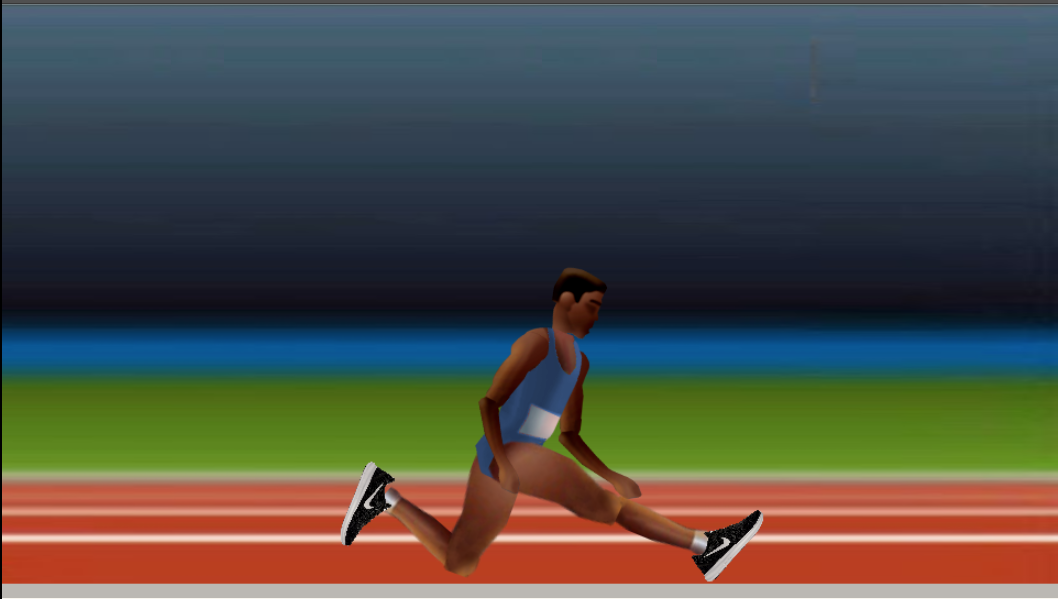
\includegraphics[scale=0.4]{Images/modelWithGraphics.PNG}}
\caption{model with graphics added}
\label{modelWithGraphics}
\end{figure}

\subsection{Game flow}
\label{sec:gameFlow}
Finally all the other components of the game were added:

\begin{enumerate}
	\item Collisions with the floor - Each limb that cannot touch the floor is put into a collision group. This group is used to check whether a collision with the floor occurs, and if so end the game.
	\item Calculation of distance reached so far - a function of the x value of the athletes torso
	\item Text showing the distance reached on the screen.
	\item Recording the high score and displaying it on the screen
	\item A User help box shown on game start-up
	\item Checking whether the user has reached the end of the 100m and displaying the congratulations message if the player gets to 100m
\end{enumerate}

\section{Implementation of evaluation software}
\label{studyimpl}

To evaluate the project, I will be analysing the results from a user study. This analysis will be happening in the evaluation section, however a large amount of work went into implementing the testing environment so I will describe that here.

The center of the study is a controlled experiment, in which participants are randomly placed into one of two groups, each of which play the two versions of QWOP in a different order.
Each game is played for 5 minutes while the key presses and distances reached for each participant are recorded.
Either side of the experiment there is a questionnaire.
% The first questionnaire finds out the demographics and previous experience of each participant. 
%The second questionnaire records the opinions of the participant through questions such as `which version did you enjoy more'. 
Next I will explain the implementation of the evaluation scaffolding used during the user study.

% breakdown of user study sections used later
% \newcommand{\userStudySections}{
% 	\begin{enumerate}
% 		\item A html page that guides the participant through the sections of the study
% 		\item An embedded Google form that finds out demographics and the previous experience of each participant.
% 		\item An A/B test. Each participant is randomly placed into one of the two groups, each of which play the two versions of QWOP in a different order. Each game is played for 5 minutes before the page moves onto the next section. While each game is played, the key presses and distances reached for each participant are recorded. The benefit of doing a randomised control trial is that selection bias is minimised. The splitting of participants into two groups means that the effect of playing one game before the other can be taken into consideration and not affect the analysis.
% 		\item A final questionnaire that gives feedback on the two versions
% 	\end{enumerate}
% }


\subsection{Web page hosting user study}
\label{sec:webPage}

To host the instrumented software I wrote a webpage that guides the users through the sections of the study. 
As I wanted to get lots of participants to take part in my user study, I wrote a web page to host the study so that participants could take part concurrently. It was also useful to host it on a web page because I can host both versions of QWOP in iframes, embed Google forms as questionnaires, and record the actions of the user. The actions of the user such as key presses and distances reached over time can be analysed along with other data to evaluate the success of the game.

images of page

\subsection{Server software to receive and store user study data}
\label{sec:serverSoftware}


I hosted the web page page on my SRCF web space. When the web page is recording data, it sends the data it has recorded to a PHP script at regular time intervals. This script records the data into separate files for each participant, so that all the data can be accessed in one place afterwards.

\subsection{Chrome extension for reading distance from QWOP}
\label{sec:chromeExtension}

% todo: Start by telling me what the problem is.  Is it that the implementation didn't expose its distance variable to something else? You see I don't understand -- and it's your job to help me feel I do understand your program, and this needs you explaining in more detail :-)
%todo: redo with alan's comments

Later on in the implementation I discovered that I couldn't access the distance that the player had reached for the original QWOP. It it impossible to access data from the game when hosting the original website inside an iframe, since all the game data is inside an anonymous function.
Unfortunately When attempting to run the game by taking the html, JavaScript and other local resources that it accessed, and running them myself, the game's canvas goes orange and the game doesn't start.
Since running an edited version of the original website did not work, I tried accessing the colour values of the game's canvas, then I could use OCR to read the distance from the screen itself. Accessing the pixel values from the canvas inside the iframe didn't work as QWOP has a OpenGL setting that made the GLBuffer unreadable.s
In the end however the distance was made accessible by creating a chrome extension that took a screenshot of the page and placed it in a canvas. Then the data collection page takes the section of the screenshot that contains the distance text, inverts the colours so that it's black text on a white background, and places it into a smaller canvas. Then a lightweight JavaScript OCR script called ocrad.js is used to to read the text. With a little editing of the script's output, it gave an accurate value.




% %%%%%%%%%%%%%%%%%%%%%%%%%%%%%%%%%%%%%%%%%%%%%%%%%%%%%%%%%%%%%%%%%%%%
% % Evaluation (eval+conc ~ 2500)
\chapter{Evaluation}
\section{Success Criteria}

%In my project proposal the success criteria is defined like so:
The project proposal talks about the aims of the project like so:

\begin{displayquote}
At the end of the project I expect to be able to demonstrate a game similar to that of the original QWOP [...] although I am not aiming to replicate the behaviour of the original QWOP exactly [...]
\end{displayquote}
\begin{displayquote}
The athlete should have the same physical qualities that make it seem human, and the game should have the same gameplay items that make it work. The Work to be done section breaks down how this will be done in more detail.
I propose to test how successful the project is with a user study. Since the quality of a game is subjective, it is appropriate to do a user study to evaluate the project.
\end{displayquote}

I shall now clarify these objectives of the project into a success criteria.
The rest of the evaluation will be aimed at showing with evidence that these criteria have been met.
The success criteria are:


\begin{enumerate} 
	\item My JavaScript version is faithful to the original QWOP; it contains the same mechanics, 
	%that the player experiences in the same way
	that gives the player a similar experience.
	\item My version will be different in some aspects, to the improvement of the game.
\end{enumerate}

Since measuring `improvement' is subjective, enjoyment of the player is a good metric to use. 
% The remake is supposed to work like the original in the way a user interacts with it and plays the game - has the same game mechanics
% but even though it should be faithful to the original in the way it works, the intent was to make it different in order that more people would find it enjoyable.
% so success is it works in a similar way, but is different in a way that makes it more fun.

% I shall now show that my project meets these objectives with the 

% the stats show that it is similar
% i made some changes to make it easier and more fun for players
% new curve
% more fun - backed up by hci stuff?


% I have undertaken a controlled experiment with instrumented software and made use of A/B testing to allow you to control for ordering effects. You have used survey methods to perform both quantitative and qualitative assessment of user perceptions of your software.

% there is conclusion to sum up?

% Sections of study in prose
To evaluate the project I have performed a user study. 
Section \ref{studyimpl} of the Implementation chapter shows the implementation of the code used in the user study.
The rest of this chapter will go into detail explaining the design choices for the user study, and analyse its results.

The center of the study is a controlled experiment. Participants are randomly placed into one of two groups, each of which play the two versions of QWOP in a different order.
Each game is played for 5 minutes while the key presses and distances reached for each participant are recorded. More detail and analysis of this data is in Section \ref{controlled experiment results}

Before the participants take part in the controlled experiment, they are asked to fill in a questionnaire asking for their demographics and previous experience of playing QWOP and other video games. After the controlled experiment, there is another questionnaire that determines the participant's opinion of the two versions they have played.
Sections \ref{q1} and \ref{q2} show the design and results of these questionnaires.


%The user study is made up of these sections, the design on which has been discussed in the implementation:

% The benefit of doing a randomised control trial is that selection bias is minimised. The splitting of participants into two groups means that the effect of playing one game before the other can be taken into consideration and not affect the analysis.

% other things that can go in
% 	demographics broad summary
% 	line graph sample
% 	3 hist

\section{Intro Questionnaire Responses}
\label{q1}

The first questionnaire asked for the demographics of each participant.
30 participants took part in the user study. This is a good number because...
Figure \ref{demographics} shows the age and gender of the participants.


\begin{figure}[tbh]
\centerline{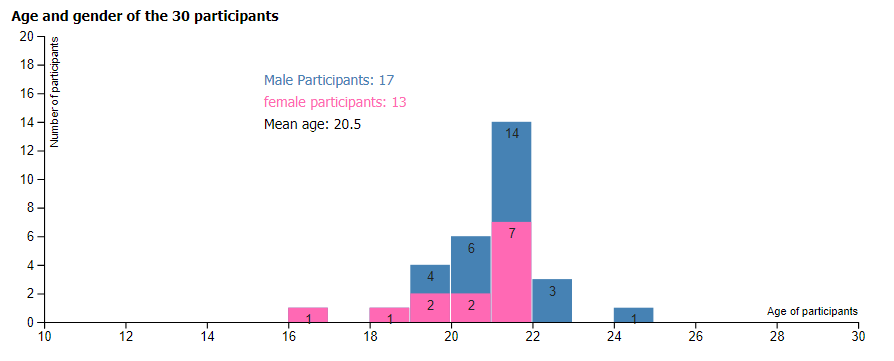
\includegraphics[scale=0.7]{participantDemographics.PNG}}
\caption{Participant demographics}
\label{demographics}
\end{figure}

The next question asked was whether the user had played QWOP beforehand, Figure \ref{previousExperienceTable} shows the options that were available to choose from and the frequency that the answers were picked.
Most of the user hadn't played QWOP before.
that matters because..???


\begin{figure}[tbh]
\begin{center}
\begin{tabular}{ |l|l| }
  \hline
  Previous experience playing QWOP   & Frequency of choice \\ \hline \hline 
  Never played before                & 19 \\ \hline
  Less than 10 minutes               & 5  \\ \hline
  Between 10 and 30 minutes          & 3  \\ \hline
  Longer than 30 minutes             & 2  \\ \hline
  A long time over multiple sessions & 1  \\ \hline
\end{tabular}
\end{center}
\caption{Previous experience of participants}
\label{previousExperienceTable}
\end{figure}


The third question asked for how long each participant plays video games during a typical week outside term time. Figure \ref{previousExperienceTable} shows the options that were available to choose from and the frequency that the answers were picked.
This matters because..???

\begin{figure}[tbh]
\begin{center}
\begin{tabular}{ |p{8cm}|c| }
  \hline
Time spent playing video games per week during a typical week outside of term time & Frequency of response \\ \hline \hline
Less than an hour      & 22 \\ \hline
Between 1 and 5 hours  & 2  \\ \hline
Between 5 and 20 hours & 4  \\ \hline
More than 20 hours     & 2  \\ \hline
\end{tabular}
\end{center}
\caption{Game playing experience of participants}
\label{gamesExperienceTable}
\end{figure}



\section{Controlled experiment results}
\label{controlled experiment results}


In this section, the controlled assessment will be explained, and the data recorded during the controlled experiment will be presented and analysed.
%While each participant plays both versions, the keys being pressed and the distance reached is being recorded. Here I shall use this data to analyse whether my version is faithful to the original, and how they compare.

During the controlled experiment each participant was randomly placed into one of two groups.
The two groups play both versions of the game with instrumented code added. This allowed me to record the keys that the participants pressed, and the distance that they had travelled over time. The implementation of the instrumented software is described in the Implementation chapter, Section \ref{studyimpl}.
Before the participants took part in the survey, they gave consent for data to be collected from their usage of the software. Consent was given when participants signed a form explaining that they understood that the software instrumented, and that the data was being collected from their usage. It also explained that they could opt out of the data collection at any point if they wished. scans of the sheets can be found at: todo
%Each participant's usage of instrumented software is recorded.
Group A played my version (version gla) first and then played the original (version fod). Group B played them in the opposite order.
Each game was played for 5 minutes. When a participant moved on to a section of the user study where one of the games is played, a timer is started. When the 5 minutes is up, the page moves onto the next section. Between the two games there is a break page where the participant can press next when they are ready for the second version.
Participants have these 5 minutes to get as far as they can. Whenever they fall over they start again and can have as many restarts as they want in the 5 minutes. Figure \ref{assorted} shows examples of the distance some of the participants reached recorded over time.
\begin{figure}[tbh]
\centerline{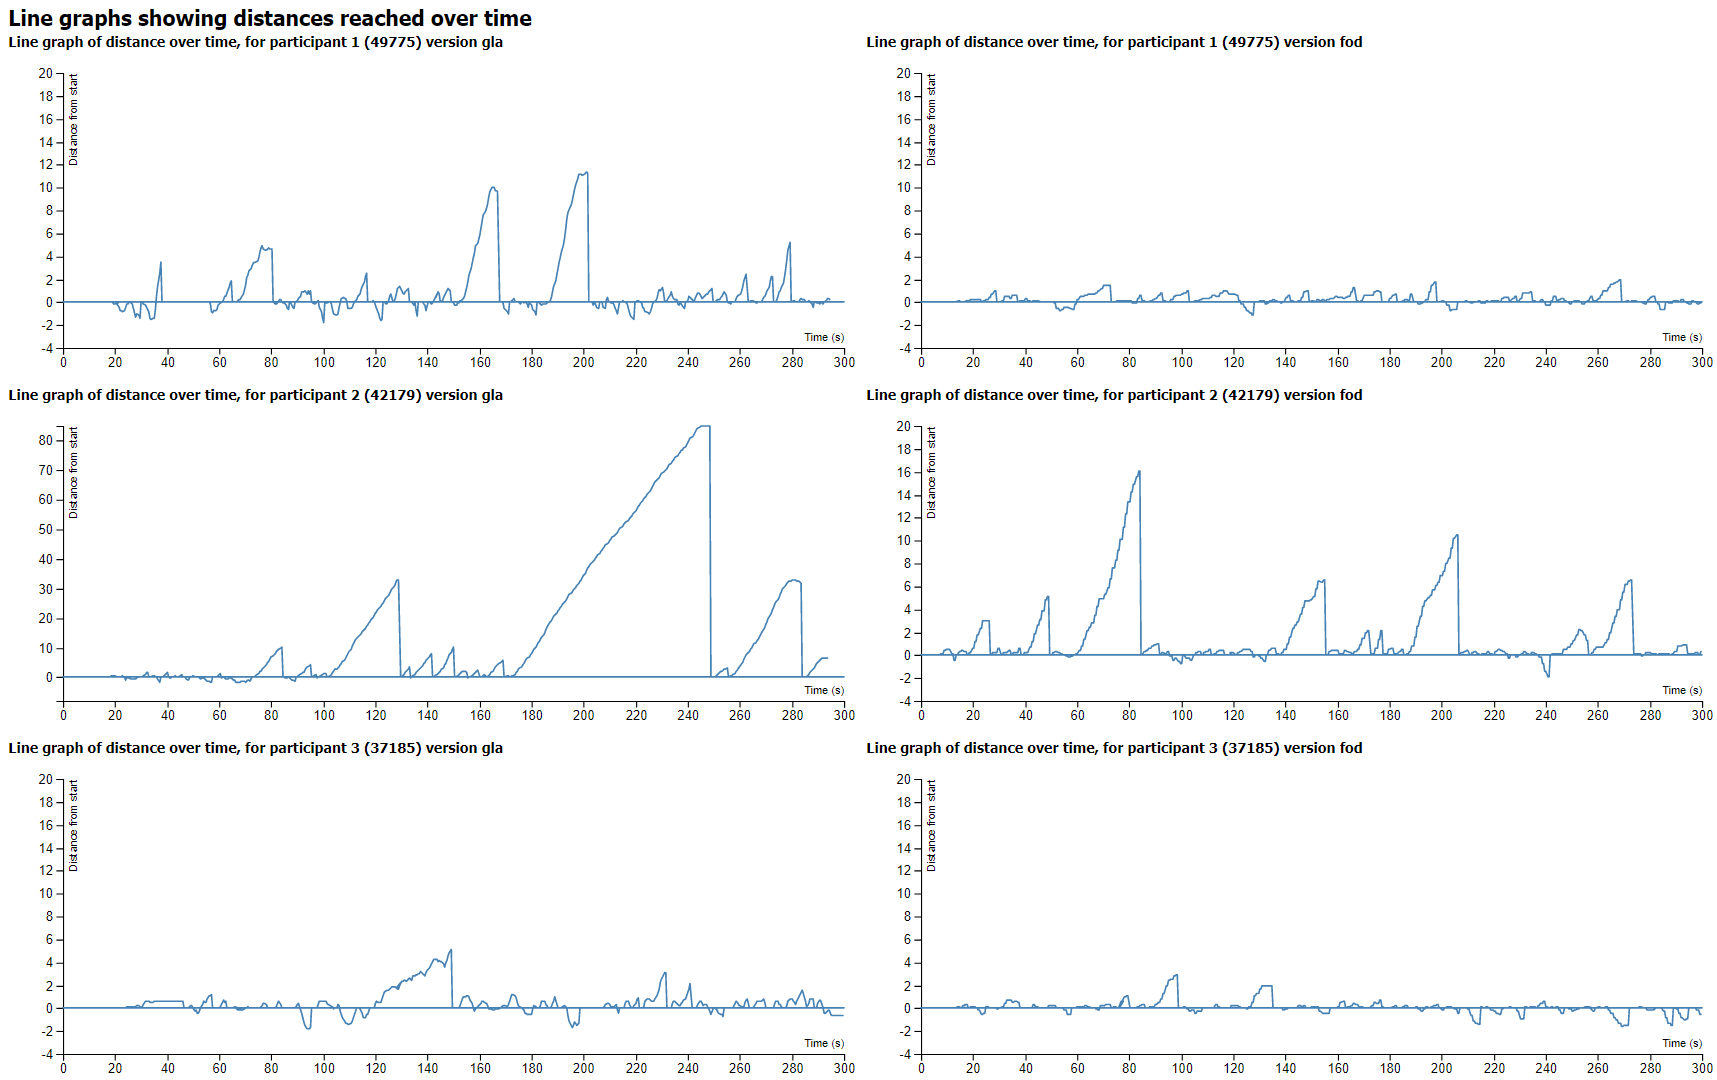
\includegraphics[scale=0.39]{assortedLineGraphs.PNG}}
\caption{A selection of Distance over time graphs}
\label{assorted}
\end{figure}


\subsection{Restart Distances}
\label{restartDistances}

In Figure \ref{assorted} one can see the participants attempt to go forward, reach a distance, and then restart. 
%Participant 2 reaches 85m at around 250 seconds.
To begin the analysis I shall compare the distances that the participants reach at the end of each run; before they fall and restart, or run out of time.
Figure \ref{glaRestarts} shows a histogram of all of these restart distances over the 30 participants for my JavaScript remake, version gla. Figure \ref{fodRestarts} shows the same but for the original QWOP, version fod.
These histograms contain all the restart distances for each version, and includes both participant groups.
The affect of the order a participant played the games is analysed later, as Section \ref{learningBias} investigates the learning bias of playing the other version first.

\begin{figure}[tbh]
\centerline{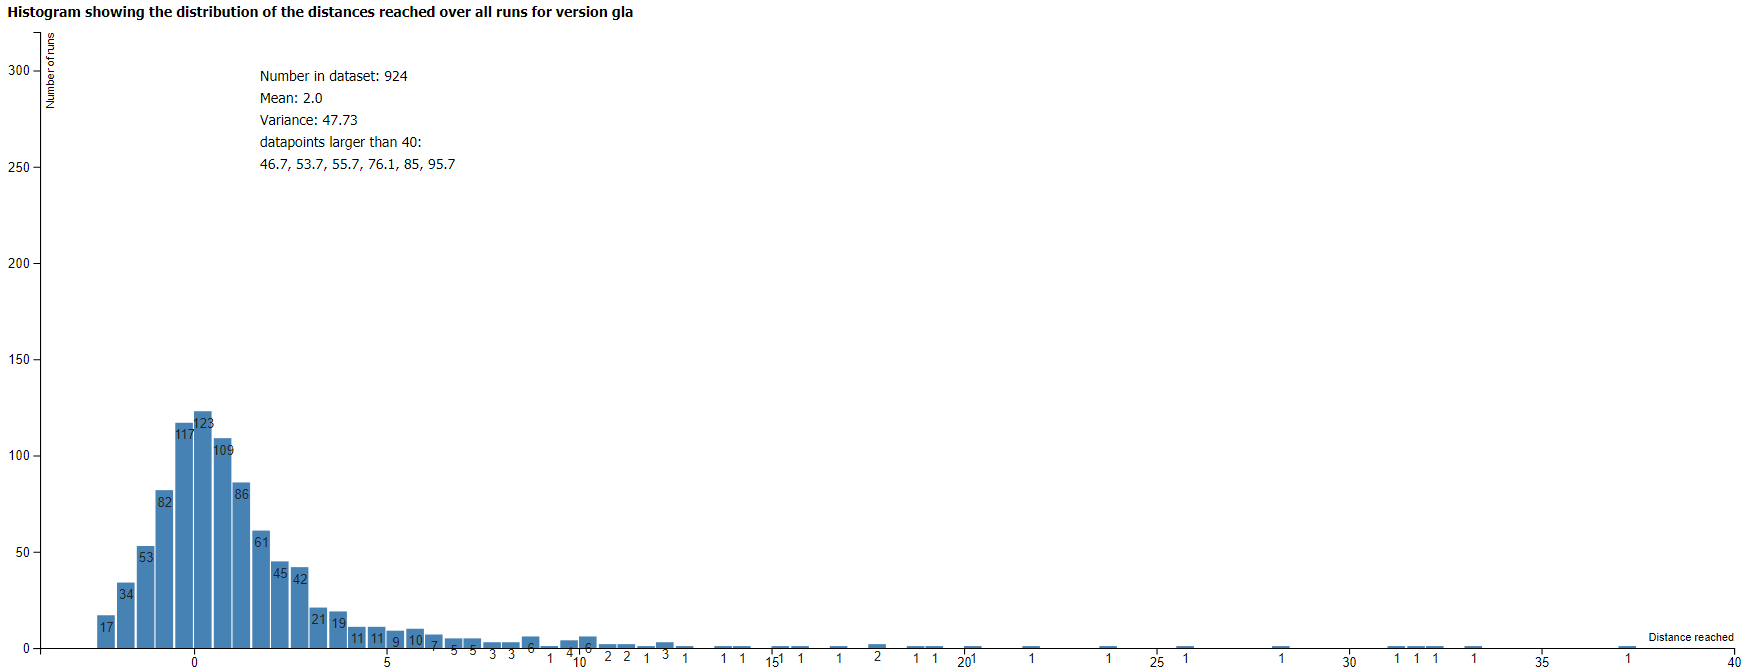
\includegraphics[scale=0.39]{glaRestarts.PNG}}
\caption{Restart distances for version gla}
\label{glaRestarts}
\end{figure}

\begin{figure}[tbh]
\centerline{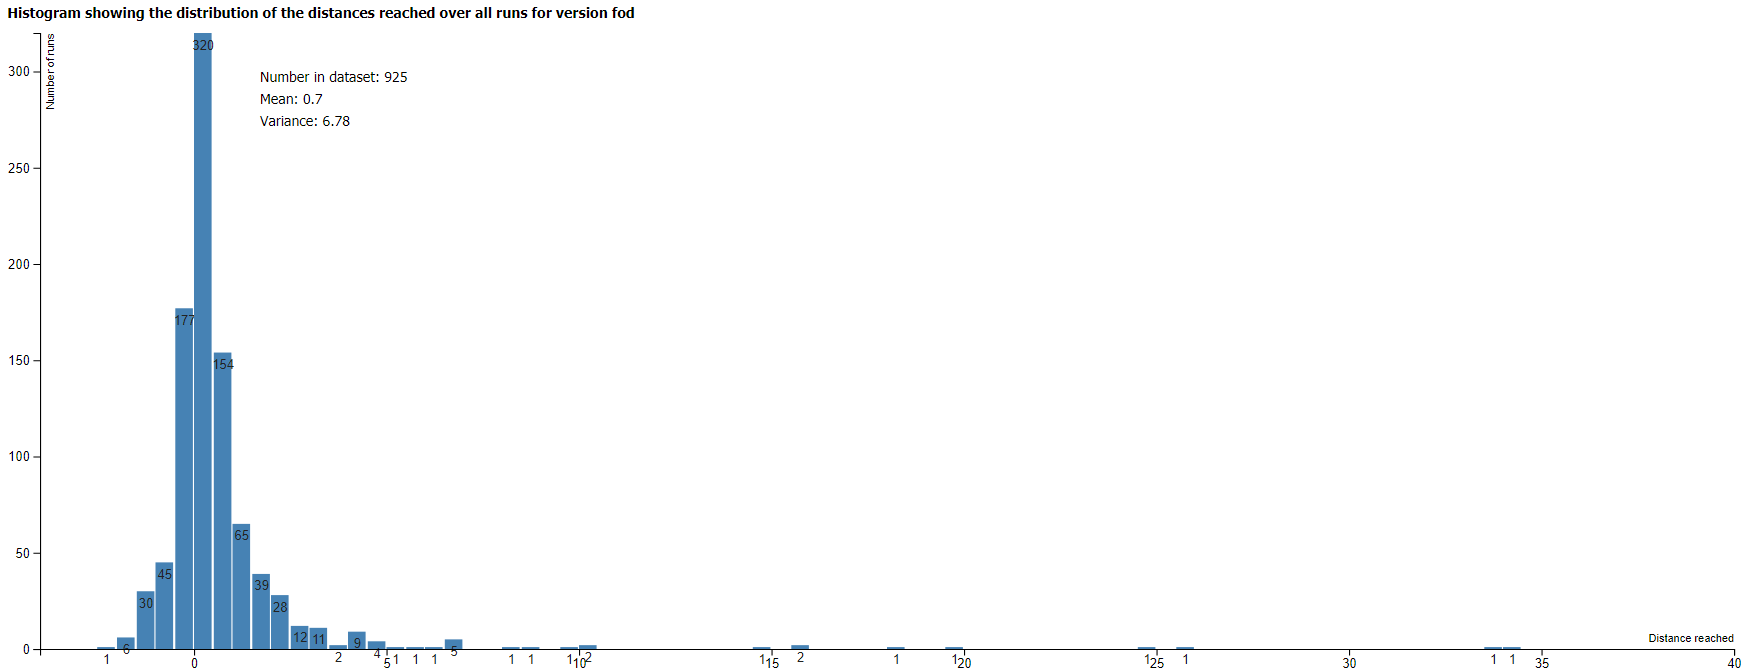
\includegraphics[scale=0.39]{fodRestarts.PNG}}
\caption{Restart distances for version fod}
\label{fodRestarts}
\end{figure}

The first thing to notice is that... good stats words
It is striking that the total number of restarts is so close. The number of runs for version gla is 924, and for version fod it is 925.
My version is very faithful to the original in this regard and it shows that their gameplay share the 

%faithful to the original.

\begin{center}
\begin{tabular}{ |p{3cm}|c| }
  \hline
Version& Average time of run (s)\\ \hline
gla & 9.74 \\ \hline
fod & 9.73 \\ \hline
\end{tabular}
\end{center}

% 300*30/924 = 9.74 gla
% 300*30/925 = 9.73 fod
% This makes the data comparable?

When comparing the restart distances of the two versions in Figure \ref{glaRestarts} and \ref{fodRestarts}, the graphs share a similar shape. As they share the same area, \ref{glaRestarts} is a stretched version of \ref{fodRestarts}

\subsection{Investigation of Learning Bias}
\label{learningBias}


%One thing you’ve not yet done in the Evaluation is see if there is a learning bias between the first and second versions the participants tried. For example, is it the case that those who used fod first, then did better at gla than those who did gla first? You should take advantage of your experimental design to test this.


\section{Second Questionnaire}
\label{q2}

The second questionnaire happens after the participants have played both versions of the game.
Here are the questions, with the figures containing the data.
and it contains the following questions aimed at comparing the two versions:

\begin{enumerate}
	\item Which version of the game do you think you were more successful at? Figure \ref{successfull}
	\item Which version felt like you had more control over the athlete? Figure \ref{opinions}
	\item Why do you think this was?
	\item Do you think playing the first version of the game improved your performance in the second version? Figure \ref{firstHelpedSecond}
	\item Which version did you enjoy more? Figure \ref{opinions}
	\item Why do you think this was?
\end{enumerate}

say about answers to choose from and why good from
%https://www.tech.cam.ac.uk/Ethics_guidance/Survey-Methods

Which version of the game do you think you were more successful at?
could look at thought vs reality but doesn't seem that useful?

Which version felt like you had more control over the athlete?
see Fig \ref{opinions} 

why ? open coding?

first improved second?

\begin{figure}[tbh]
\begin{center}
\begin{tabular}{ |p{6cm}|c|c|c| }
  \hline
Opinion whether playing the first& \multicolumn{3}{|c|}{Frequency of response} \\ \cline{2-4}
helped improve the second& Group A& Group B&Total\\ \hline
Definitely     & 1 & 5 & 6 \\ \hline
Maybe          & 5 & 7 & 12\\ \hline
I'm not sure   & 3 & 0 & 3 \\ \hline
Maybe not      & 3 & 0 & 3 \\ \hline
Definitely not & 3 & 3 & 6 \\ \hline
\end{tabular}
\end{center}
\caption{Participant opinion of whether playing the first game helped improve their score for the second, by group.}
\label{firstHelpedSecond}
\end{figure}


\begin{figure}[tbh]
\begin{center}
\begin{tabular}{ |p{6cm}|c|c|c| }
  \hline
Version& \multicolumn{3}{|c|}{Frequency of response} \\ \cline{2-4}
& Group A& Group B&Total\\ \hline\hline
First played   & 8 & 5  & 13 \\ \hline
Second played  & 7 & 10 & 17 \\ \hline\hline
Version gla    & 8 & 10 & 18 \\ \hline
Version fod    & 7 & 5  & 12 \\ \hline
\end{tabular}
\end{center}
\caption{Participant opinion of whether they were more successful at the first or second version.}
\label{successfull}
\end{figure}



\begin{figure}[tbh]
\begin{center}
\begin{tabular}{ m{4cm}|c|c|c|c||c|c||c|c| }
\cline{2-9}
 & \multicolumn{2}{|c|}{Group A} & \multicolumn{2}{|c|}{Group B} & \multicolumn{4}{|c|}{Total over groups} \\
\cline{2-9}
% Which version...&First (gla)&Second (fod)&First (fod)&Second (gla)&gla&fod&First&Second \\ \hline
&First &Second &First &Second &&&& \\
&version &version &version &version &gla&fod&First&Second \\
&(gla)&(fod)&(fod)&(gla)&&&& \\ \hline
\multicolumn{1}{ |m{4cm}| }{Which version felt like you had more control over the athlete?}& 7 & 8 & 4 & 11 & 18 & 12 & 11 & 19 \\ \hline
\multicolumn{1}{ |m{4cm}| }{Which version did you enjoy more?}   & 9 & 6 & 5 & 10 & 19 & 11 & 14 & 16  \\ \hline
\end{tabular}
\end{center}
\caption{Results of participant choice of version}
\label{opinions}
\end{figure} 







% %%%%%%%%%%%%%%%%%%%%%%%%%%%%%%%%%%%%%%%%%%%%%%%%%%%%%%%%%%%%%%%%%%%%
% % Conclusion (eval+conc ~ 2500)
% \chapter{Conclusion}
% \section{section 1}
% Conclusion





\end{document}
